\documentclass[11pt]{article}
\usepackage{eacl2009}
\usepackage{times}
\usepackage{url}
\usepackage{latexsym}

\setlength{\intextsep}{1ex}

\usepackage{graphics}
\usepackage[utf8x]{inputenc}
\usepackage{ucs} %sami letters\renewcommand
%\usepackage{covington} % ling examples

%\usepackage{linguex}
%{\refdash}{}
%\usepackage[T1]{fontenc}
%\usepackage{multirow}
%\usepackage{tabularx} %specified width
\begin{document}

\title{Constraint Grammar in Dialogue Systems}

\author{Lene Antonsen\\
  University of Tromsø\\
  Norway\\
  {\tt lene.antonsen}\\{\tt @uit.no}  \And
  Saara Huhmarniemi\\
  University of Tromsø\\
  Norway\\
  {\tt saara.huhmarniemi}\\{\tt @helsinki.fi}  \And
  Trond Trosterud\\
  University of Tromsø\\
  Norway\\
  {\tt trond.trosterud}\\{\tt @uit.no}}


%\date{}

\maketitle
\pagenumbering{arabic}

% tt:
% Adding notes for further consideration:
% This paper will differ from the Oahpa_nodalida paper in being more CG focused.
% Issues:
% Probably skip the Sentence generator section.
% Discuss the CG rules more thoroughly
% Do more out of the evaluation:
% - Go through all accepted Sahka sentences, and study the recall:
%   Is the program able to catch:
%   - all targeted errors?
%   - some non-targeted errors?
%   ... and precision:
%   - how do we fare with the non-accepted sentences, are they really errors?

 
\maketitle

\begin{abstract}
This article discusses the use of Constraint Grammar as the parser engine in parser-based CALL programs for North Sámi. The parser locates grammatical errors in a question-answer program and a dialogue program, and the parser is also used for navigating inside the dialogue.

%Special focus is given to the relaxation of the ordinary disambiguator, the error-detecting rule set, and recall and precision of the error detection.
\end{abstract}

\section{Introduction} 

The present paper discusses the use of vislcg3 in two different dialogue systems for learning North Sámi: \textit{Vasta} -- a QA-drill with open questions, and \textit{Sahka} -- a  dialogue between program and user within a scenario. The underlying pedagogical goal for both is exercising verb inflection, choosing the correct case and extending the learner's vocabulary. 

Vislcg3 is used both for adding feedback about grammatical errors, for navigating in the \textit{Sahka}-dialogue based on the user's answers and for identifying what parts of the user answer to use in further questions.

Our leading idea was to utilize the existing analyser for Sámi when developing pedagogical programs for language instruction. With vislcg3 we had the possibility of making an intelligent tutoring system with sophisticated error analysis where student tasks could go beyond multiple-choice or string matching algorithms. 

Sámi is a language with complex morphology, and it demands much practising before the student reaches necessary skills. But as a minority language Sámi does not everywhere provide enough opportunities to practise the language in a natural way. There is also a lack of teaching materials. Because of that, programs accessible on the Internet may be a supplement to the instruction given at school or in university. 

\section{Basic grammatical analysis}
The basic grammatical analysis of North Sámi is done with fst and a constraint grammar parser made at UiT. The relevant resources are the following:

\begin{itemize}
\item a morphological analyser/generator with finite state transducers, compiled with the Xerox compiler xfst.  
\item a morphological disambiguator based on constraint grammar with 3300 manually written rules and a syntactic analyser which adds grammatical function (vislcg3). 
\end{itemize}

\section{Sentence generator}
The question-answer drill \textit{Vasta} has randomly chosen questions, yes/no-questions and wh-questions. In order to be able to create a large number of potential tasks, we implemented a sentence generator. With the generator we can easily offer variation to the user, instead of tailoring every task with ready-made questions.

The matrix contains two types of elements: constants and grammatical units. The selection of words from the pedagogical lexicon is constrained by semantic sets. The pedagogical lexicon forms a collection of words that are considered relevant for the learners of North Sámi in schools and universities. The dialectal variation is taken into account in the lexicon as well as in the morphological generator, so the user can choose eastern or western dialect for the tasks. The sentence generator handles agreement e.g. between subject and the main verb. 

\begin{figure}%[tbp]
\begin{center}
\scalebox{.42}[.42]{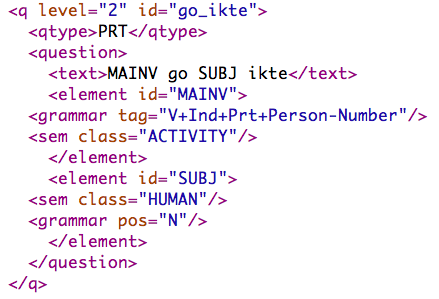
\includegraphics{presentation/img/sentencegenerator.png}}\\
\caption{A sentence generator template consisting of constants and grammatical units (MAINV question-particle SUBJ yesterday).}
\label{sentgen}
\end{center}
\end{figure}

In Figure \ref{sentgen} is an example of a question template in which the main verb (MAINV) is fixed to past tense, but the person and number inflection may vary freely. In Figure \ref{vastasent} is the template realised as a task in \textit{Vasta}. The question matrices are marked with level, so there is a level option. There are 111 matrix questions.

\begin{figure}%[tbp]
\begin{center}
\scalebox{.35}[.35]{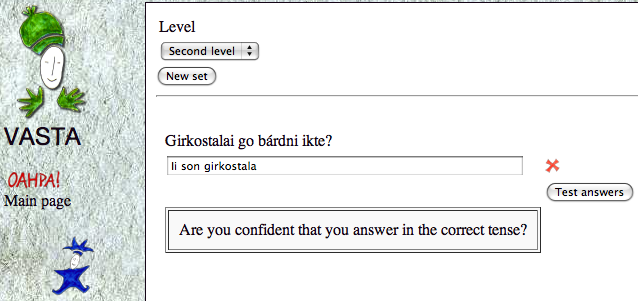
\includegraphics{presentation/img/Vasta_sentencegen_example.png}}\\
\caption{A generated question and a student's answer in \textit{Vasta}. ("Did the boy go to church yesterday?" 
"No, he does not.")}
\label{vastasent}
\end{center}
\end{figure}
 
\section{Analysing the syntax of the user's answer} 
We use vislcg3 for analysing the user's input. First there is a rule set, which disambiguates the user's input only to a certain extent. The rule set is relaxed compared to the ordinary disambiguator, in order to be able to detect the relevant readings despite of a certain degree of grammatical and orthographic errors in the input. The last part of the file consists of rules for giving feedback to grammatical errors, and rules for navigating to the correct next question or utterance of in the dialogue, due to the user's answer.  

The system question and user answer pairs are merged, and given to the analyser as one text string. The question mark in the question is exchanged for a special symbol ("qst" QDL). We use this symbol, rather than the question mark itself, in order not to introduce a sentence delimiter in the analysis, since we want to refer to the question and the answer separately in the rules (left or right side of the QDL), but also treat the question-answer part as one unit. Many of the constraints are based on the grammar and semantics in the question -- e.g. the tense and person inflection of the verb, the case of NP in the answer and so on. The question itself restricts the possible interpreting of the input.

Should we mention that vislcg3 is also used for free input in one VISL program?

\begin{figure}%[tbp]
\begin{center}
\scalebox{.40}[.40]{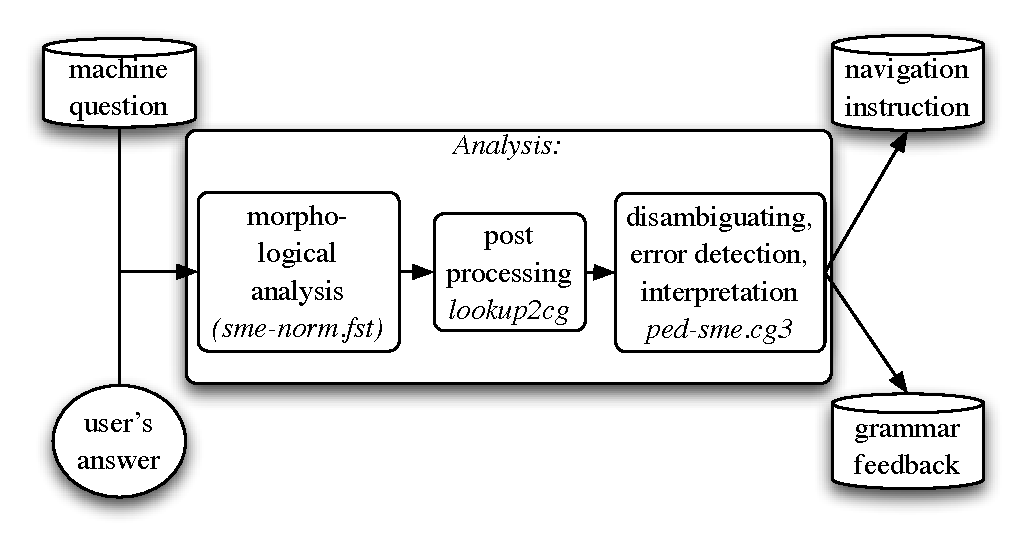
\includegraphics{presentation/img/qa2.pdf}}\\
\caption{Schematical view of the process}
%\label{nounlex}
\end{center}
\end{figure}


\subsection{Navigating in the dialogues}
In the \textit{Sahka} dialogues the user may exercise Sámi in a quite natural way and therefore the user's input also needs tags for navigation in the dialogue itself so the user gets correct respons to her answer.

The questions in the dialogues are not generated, but written. Every question has its own unique name, so we can link to it from another questions, and it is also possible to make a CG-rule for specific questions.  

To show how it works, we can jump into a dialogue in \textit{Sahka}. In Figure \ref{sahka} the setting is a visit at a friend who has moved into a new flat, and she needs a helping hand with moving the furniture into the rooms. We have come to the third question – and the user gets grammatical feedback as well as that the navigation in the dialogue is due to the answer. In Figure \ref{hivssetanalysis} the analysis assigns both grammatical error tag and navigation tag to the question-answer pair. The rule for the navigation tag is in Figure \ref{hivssettag}.
 

\begin{figure}%[tbp]
\begin{center}
\scalebox{.25}[.25]{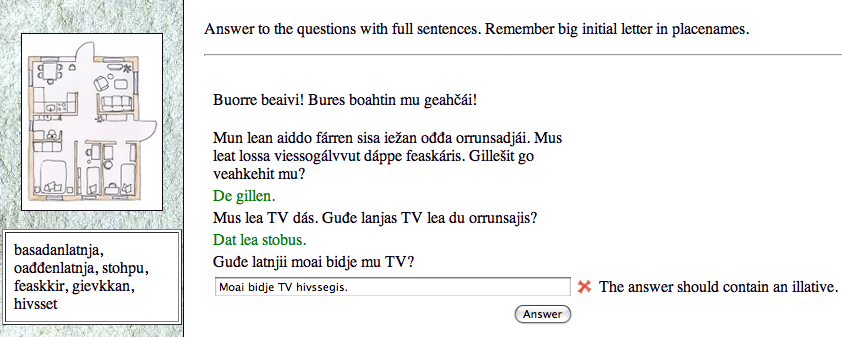
\includegraphics{presentation/img/TVhivssegis.png}}\\
\caption{From \textit{Sahka}. Question: "In which room should we place the TV?" Student: "We should place it in the toilet."
}
\label{sahka}
\end{center}
\end{figure}


\begin{figure}%[tbp]
\begin{center}
\scalebox{.40}[.40]{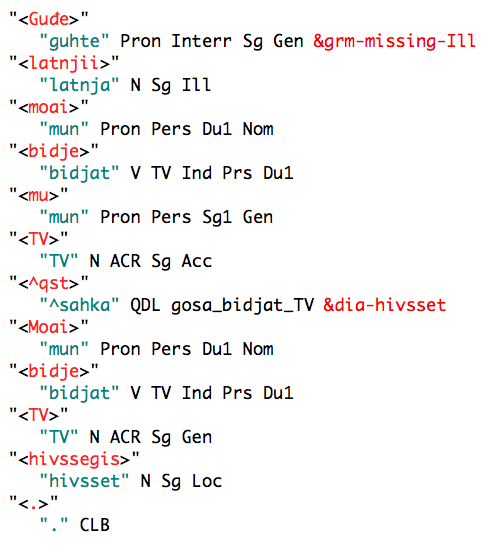
\includegraphics{presentation/img/hivssegisCGanal.png}}\\
\caption{Assignment of tags}
\label{hivssetanalysis}
\end{center}
\end{figure}

\begin{figure}%[tbp]
\begin{center}
\scalebox{.35}[.35]{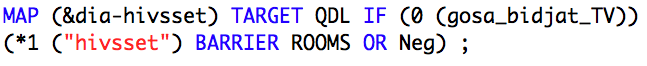
\includegraphics{presentation/img/hivsset_tag.png}}\\
\caption{Rule for assignment of navigation tag. This is a rule for the question with id 'gosa\_bidjat\_TV' if the answer is 'toilet'.}
\label{hivssettag}
\end{center}
\end{figure}



\begin{figure}%[tbp]
\begin{center}
\scalebox{.5}[.5]{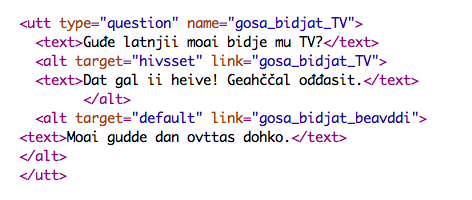
\includegraphics{presentation/img/gosabidjatTV.png}}\\
\caption{Question: "In which room should we place the TV?"
Alt. WC: "That is not a good idea. Make a new try." 
Default: "We carry it there together." 
}
\label{altlinks}
\end{center}
\end{figure}

In Figure \ref{altlinks} there are two alternative links for the answers to the question. One of them is connected to the \&dia-hivsset tag and will give the answer “That is not a good idea. Make a new try.” The other link is default. 

Every question has its own unique id, which is used in navigating between questions. In addition, the CG-rules may be tailored for specific questions.  

Many of the rules are general rules, e.g. the input is tagged during analysis with information on whether it is interpreted as affirmative or negative, as in Figure \ref{afforneg}.

There are also rules if there is semantic information, which is assigned with a target tag. In Figure \ref{targettag} is a general target rule for question which require an answer in accusative. The choice of alternative links is dependent upon what kind of tag the question-answer pair gets. There will always be a default link in case there will not be any tag. 
 

\begin{figure}%[tbp]
\begin{center}
\scalebox{.3}[.3]{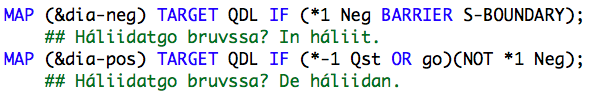
\includegraphics{presentation/img/aff_or_neg_colours.png}}\\
\caption{Tags for affirmative and negative answer. 
}
\label{afforneg}
\end{center}
\end{figure}

\begin{figure}%[tbp]
\begin{center}
\scalebox{.3}[.3]{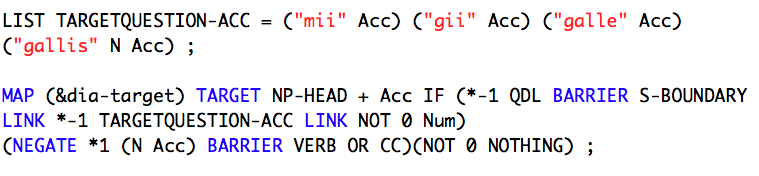
\includegraphics{presentation/img/target_acc.png}}\\
\caption{Assignment of target tag for answer in accusative. 
}
\label{targettag}
\end{center}
\end{figure}

In addition, a special tag indicates whether the sentence contains some information that should be stored. The program is thus able to store simple information such as the student’s name, place where she lives and for example the type of her car, like in Figure \ref{nametag}, and use this information in tailored questions or utterances.

\begin{figure}%[tbp]
\begin{center}
\scalebox{.3}[.3]{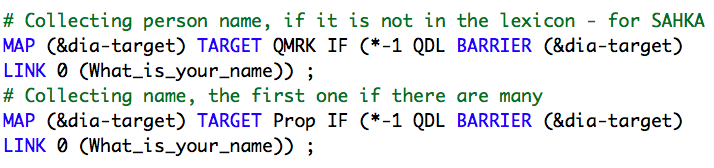
\includegraphics{presentation/img/picking_name_new.png}}\\
\caption{Collecting information from the input for storing. 
}
\label{nametag}
\end{center}
\end{figure}

To many yes/no questions it can be natural to answer more than only yes/no. E.g. Do you have children? the student can answer 'Yes, I have two children.' It gives then a bad impression if the next question is 'How many children do you have?'. To prevent that we have a pass-tag for omitting the next question, as in Figure \ref{omit}.

\begin{figure}%[tbp]
\begin{center}
\scalebox{.4}[.4]{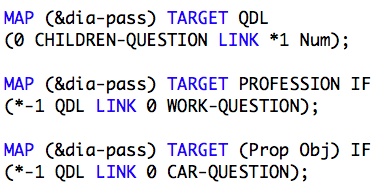
\includegraphics{presentation/img/pass_rules.png}}\\
\caption{Tag for omitting the next question. 
}
\label{omit}
\end{center}
\end{figure}

 
 
Some dialogues are branched according to how the user answers, e.g. if the question is about having a car, a positive answer will navigate to a branch with follow-up questions. In the same way an answer from the user about his/her age will induce a tag, which is used to navigate to different branches of the dialogue based on the age of the user, as in Figure \ref{agebranches}. The tag for age is assigned with a regex inside a CG-rule, as in Figure \ref{agerule}.



The vislcg3 also assigns target-tags as in Figure \ref{targettag}, so that the system can pick up e.g. the name of the user, a place name, his/her car make and so on, and use it in the program's questions or utterances.


\begin{figure}%[tbp]
\begin{center}
\scalebox{.35}[.35]{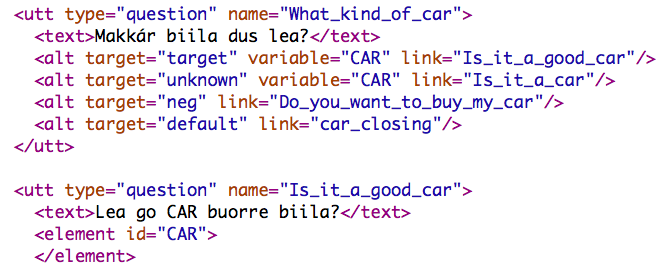
\includegraphics{presentation/img/what_car.png}}\\
\caption{Using the information.}
%\label{nounlex}
\end{center}
\end{figure}

\begin{figure}%[tbp]
\begin{center}
\scalebox{.4}[.4]{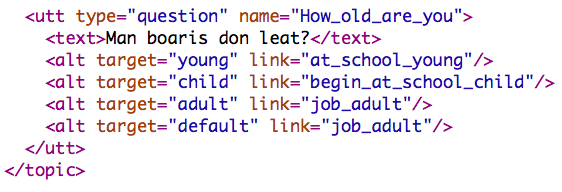
\includegraphics{presentation/img/age_branching.png}}\\
\caption{Alternative branches}
\label{agebranches}
\end{center}
\end{figure}

\begin{figure}%[tbp]
\begin{center}
\scalebox{.3}[.3]{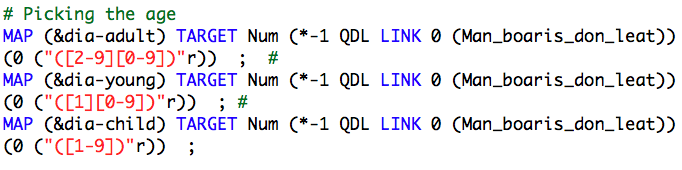
\includegraphics{presentation/img/pickingage_colours.png}}\\
\caption{Rules for age.}
\label{agerule}
\end{center}
\end{figure}

\newpage

\subsection{Tutorial feedback}
Tutorial feedback is feedback about grammar errors, and is used both in \textit{Vasta} and in \textit{Sahka}. The system uses CG-rules for assigning a tag to grammatical errors in the input. The tag generates feedback to the user. It should be noted that the system uses the grammatical analyser on the fly, exploiting full lexicons. This allows the user's answer to contain any Sámi word, also words that are not restricted to the pedagogical lexicon.

\begin{figure}%[tbp]
\begin{center}
\scalebox{.4}[.4]{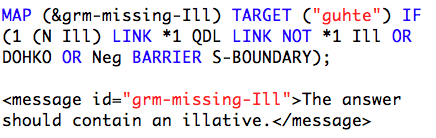
\includegraphics{presentation/img/missingIll.png}}\\
\caption{Assignment of grammar tag}
%\label{nounlex}
\end{center}
\end{figure}


The users should inflect the finite verb correctly and choose the correct case form. A a main rule, the user has to use a full sentence (containing a finite verb), and use the same verb as in the question. The CG-rule, which controls the choice of verb for the answer, uses a regular expression-based tag (a so-called sticky tag). Pro-verbs get a special treatment, so that a question containing a pro-verb will accept any verb in the answer. ORTH-VARIATION

For some of the questions in the \textit{Sahka} dialogue these requirements are somewhat relaxed. E.g. the question "What is your name?" will more naturally be answered without a verb. 

\begin{figure}%[tbp]
\begin{center}
\scalebox{.3}[.3]{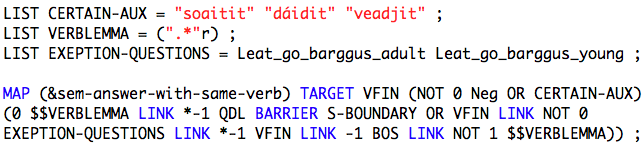
\includegraphics{presentation/img/verblemma.png}}\\
\caption{Answer with the same verb.}
%\label{nounlex}
\end{center}
\end{figure}


In \textit{Vasta} the pronouns are not allowed to be interpreted inclusively -- \textit{we — you}, not \textit{we — we}, but in \textit{Sahka} they follow the logic of the scenario.

For some questions in the \textit{Sahka}-dialogues which are made for special grammatical training, there are a whole section of rules in the vislcg3 file, for adding specific feedback to the possible errors.

The user will get only one feedback at a time, so the error tags are ordered partly a natural progress for error correction, and partly according to the likeliness of the error. First of all the user will get feedback about spelling errors. If there is not agreement between subject and verb, then s/he will get feedback on the verb form, and not on the pronoun, given the assumption that the error is in the verb form rather than in the pronoun.

The biggest problem is the user's misspellings. If the spelling error gives rise to a non-existing word form, then the message to the user is "The word form is not in our lexicon, can it be a spelling error?" 
%Here, our program is clearly inferior to a human reader, who would be able to read in a robust way, and detect what the user intended to write. Simulating this ability is not an easy task.)) 
Running the feedback through an ordinary speller engine is not a good solution, since the speller will come up with a large number of suggestions, without being able to choose between them. A possible solution would be to run a morphological analysis on the speller suggestions, and let a CG component pick the most likely candidates. PROBLEM: DIVVUN MADE FOR NATIVE SPEAKERS

The misspelling can also give rise to another word form of the same lemma. For such cases we make rules based on context. A more difficult problem emerges when the spelling error gives rise to an unintended lemma. Then the challenge is to give a feedback according to what the user think s/he has written. Feedback has to be tailored from what we know about the user’s interlanguage – and we make rules for sets of typical unintended lemmas. EXAMPLES

We are also trying to add rules in the twol-file for typical spelling errors in e.g. place names, in order for the system to give a specific feedback. The user may write a place name not found in the lexicon. Therefore it would be an improvement if the system could recognize misspellings of the names, which are in the lexicon.

NAMES as string , not analysed

Metacomments:\\
"Answering \textit{I-don't-know} is too simple. Try again."\\
"Your answer must always contain a finite verb. Could there be a typo in the verbform?"\\
"You must use one of the words in the wordlist in the left margin."\\
"You have not used the correct adjective. Try again." \\
The user can quit the dialogue in a proper way by using the verb "heaitit" (= to quit) -- then the system navigates to the closing utterance of the dialogue (to be implemented)\\

Grammar errors we have rules for:\\
verbs: finite, infinite, negative form, correct person/tense according to the question\\
case of argument based upon the interrogative \\
case of argument based upon valency\\
locative vs. illative based upon movement\\
subject/verbal agreement\\
agreement inside NP \\
numeral expressions: case and number  \\
PP: case of noun, pp based upon the interrogative \\ 
time expressions \\
special adverbs  \\
particles according to word order \\
comparision of adjectives\\

\section{Evaluation}
 
The system has identified an error in the user's input:
\begin{table}
\begin{tabular}{|l|c|c|c|}
\hline 
\textbf{Rule type}  & \textbf{corr.} & \textbf{wrong}   & \textbf{corr. \% }  \\
\hline 
wrong tense         & 7     & 0     & 100,0     \\ 
wr. V after neg   & 3     & 0     & 100,0     \\ 
no infinite V       & 1     & 0     & 100,0     \\ 
\hline 
orth. error         & 44    & 2     & 95,7      \\
wr. case V-arg  & 26    & 4     & 86,7      \\
no finite verb        & 19    & 4     &  82,6 \\
\hline 
wr. S-V agreem.   & 17    & 8     & 68,0 \\
wrong V choice        & 7     & 4     & 63,6 \\
\hline 
wrong word            & 4     & 4     & 50,0 \\
wr. case after Num  & 1     & 1     & 50,0 \\
\hline
\end{tabular}
\end{table}


Which rules are not in use? Why? \\
agreement inside NP (except for numeral expressions) \\
PP: case of noun, pp based of the interrogative  \\
time expressions \\
particles according to word order \\

\begin{figure}%[tbp]
\begin{center}
\scalebox{.35}[.35]{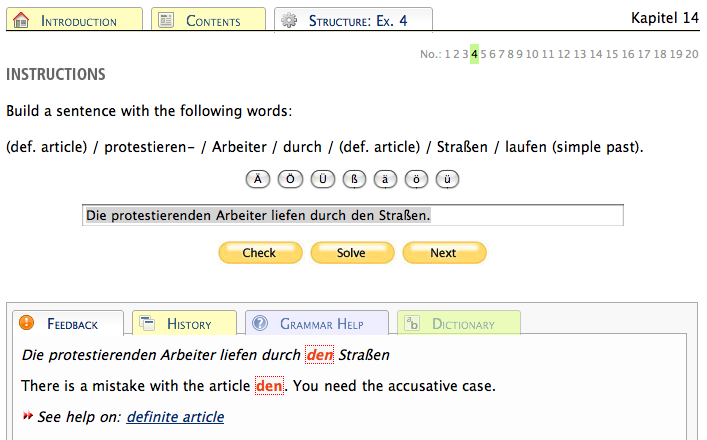
\includegraphics{presentation/img/e-tutor.png}}\\
\caption{An alternative to free input: http://e-tutor.org/}
%\label{nounlex}
\end{center}
\end{figure}
 
Precision and recall
\begin{table}%[htdp]
%\caption{default}
%\begin{center}
\begin{tabular}{|l|r|r|r|r||r|r|r|r|r|}
\hline
Type	& tp		& fp		& tn		& fn	& prec	 & rec.	& acc.	& F-ms. \\
\hline
Gramm.    &   641   &   234   &   769    &   7    &   0,73   &   0,99   &   0,85   &   0,84	  \\
Sem.       &   805   &   69    &   764    &   12   &   0,92   &   0,99   &   0,95   &   0,95		  \\
Orth.      &   875   &   0     &   776    &   0    &   1      &   1      &   1      &   1					  \\
Other      &   695   &   180   &   751    &   25   &   0,79   &   0,97   &   0,88   &   0,87	  \\
\hline
  &   3016  &   483   &   3060   &   44   &   0,86   &   0,98   &   0,92   &   0,92			  \\
\hline
\end{tabular}
%\end{center}
%\label{default}
\end{table}%

The high recall compared to the somewhat lower precision indicates that the system is a bit too critical towards the students:
It almost never lets through a (targeted) mistake, with the price of flagging some correct answers as errors.
 
 

\section{Future perspectives}
How to improve the system? \\
speller for misspellings  \\
grammartasks a la \textit{e-tutor}? \\
Vasta: decide what words the user should use, ala e-tutor as a supplement \\
Vasta: the user can choice topic instead of grammar tasks \\
Make the programs for more sámi languages \\
Classroom studies \\

\section{Conclusion}

By using a sloppy version of the syntactical analyser for North Sámi, combined with a set of error-detection rules, we have been able to build a flexible CALL resource. \\ 
The precision is not good enough  \\
We need some kind of speller or a sloppy fst with errortags \\
"Totally" free input not always the best \\




The paper shows how we have used vislcg3 for pedagogical dialogue systems for Sámi language. Vislcg3 is used in many ways: By relaxing the analysis of the input string, we are able to find errors made by the user, and assign feedback tags to analyse. Secondly, by analysing the semantics in the user's input, and assign semantic tags to the input, we are able to navigate through the dialogue according to user feedback. And finally, we can assign tag to information in the user's input and use it in the program's questions or utterances.  

The CG formalism has a great potential for use in pedagogical settings.
It is robust enough to handle erroneous data, and at the same time flexible enough to give both general corrections, and corrections targeted at specific words in specific settings.

We have seen that a major problem is spelling errors. Whether CG is able to offer a solution for this problem as well, remains a topic for future research.


\begin{thebibliography}{}

\bibitem[\protect\citename{{Beesley and Karttunen}}2003]{BeesleyKarttunen:03}
{Kenneth R. Beesley and Lauri Karttunen}.
\newblock 2003.
\newblock {\em Finite State Morphology}.
\newblock CSLI publications in Computational Linguistics.
\newblock USA.
%Bick, Eckhard (2003-8). "A Constraint Grammar Based Question-Answering System for Portuguese". In: Fernando Moura Pires & Salvador (eds.) Progress in Artificial Intelligence (Proceedings of EPIA'2003, Beja, Dec. 2003), pp. 414-418. Springer

\bibitem[\protect\citename{Bick}2003]{Bick:03}
{Eckhard Bick}.
\newblock 2003.
\newblock {PaNoLa: Integrating Constraint Grammar and CALL applications for Nordic languages}.
\newblock Holmboe, Henrik (ed.): {\em Nordic Language Technology, Årbog for Nordisk Sprogteknologisk Forskningsprogram 2000-2004}.
\newblock {183--190},
\newblock København: Museum Tusculanums Forlag.

\bibitem[\protect\citename{Bick}2005]{Bick:05}
{Eckhard Bick}.
\newblock 2005.
\newblock {Live use of Corpus data and Corpus annotation tools in CALL: Some new developments in VISL}.
\newblock Holmboe, Henrik (ed.): {\em Nordic Language Technology, Årbog for Nordisk Sprogteknologisk Forskningsprogram 2000-2004},
\newblock {171--185}.
\newblock København: Museum Tusculanums Forlag.

%\bibitem[\protect\citename{Bick}2005b]{Bick:05b}
%{Eckhard Bick}.
%\newblock 2005b.
%\newblock {Grammar for Fun: IT-based Grammar Learning with VISL}.
%%\newblock {49--64},
%\newblock Henriksen, Peter Juel (ed.): {\em CALL for the Nordic Languages.}
%\newblock Copenhagen Studies in Language 30:49--64.

\bibitem[\protect\citename{Gamper and Knapp}2002]{Gamper:02}
{Johann Gampfer and Judith Knapp}.
\newblock 2001.
\newblock {A review of intelligent CALL systems}.
\newblock {\em Computer Assisted Language Learning} 
%\newblock {329--342},
\newblock {15(4):329--342.}
%\newblock Routledge.


\bibitem[\protect\citename{Heift}2001]{Heift:01}
{Trude Heift}.
\newblock 2001.
\newblock {Intelligent Language Tutoring Systems for Grammar Practice}.
\newblock {\em Zeitschrift fur Interkulturellen Fremdsprachenunterricht [Online] }
\newblock {6(2).}



\bibitem[\protect\citename{Heift and Nicholson}2001]{Heift:02}
{Trude Heift and Devlan Nicholson}.
\newblock 2001.
\newblock {Web Delivery of Adaptive and Interactive Language Tutoring}.
%\newblock {310--325},
\newblock {\em International Journal of Artificial Intelligence in Education}
\newblock {12(4):310--325.}

\bibitem[\protect\citename{Heift and Schulze}2007]{Heift:07}
{Trude Heift and Mathias Schulze}.
\newblock 2007.
\newblock {\em Errors and intelligence in computer-assisted language learning: parsers and pedagogues}.
\newblock Routledge studies in computer-assisted language learning 2. 
\newblock New York : Routledge.

\bibitem[\protect\citename{Karlsson et. al}1995]{Karlsson:95}
{Fred Karlsson and Atro Voutilainen and Juha Heikkilä and Arto Anttila}.
\newblock 1995.
\newblock {\em Constraint grammar: a language-independent system for parsing unrestricted text}.
\newblock Mouton de Gruyter.


%\bibitem[\protect\citename{Samuelsson and Voutilainen}1997]{SamuelssonVoutilainen:97}
%{Christer Samuelsson and Atro Voutilainen}.
%\newblock 1997.
%\newblock Comparing a Linguistic and a Stochastic Tagger
%\newblock {\em Proceedings of the 35th Annual Meeting of the Association for Computational Linguistics}.
%\newblock {Association for Computational Linguistics},
%\newblock {246--253},
%\newblock {http://www.aclweb.org/anthology/P97-1032}


\bibitem[\protect\citename{{Trosterud}}2007]{Trosterud:07}
{Trond Trosterud}.
\newblock 2007.
\newblock {\em Language technology for endangered languages: Sámi as a case study}.
\newblock http://giellatekno.uit.no/background/rvik.pdf
\newblock University of Tromsø, Norway.

\bibitem[\protect\citename{{visl}}2008]{Visl:08}
{VISL-group}.
\newblock 2008.
\newblock {\em Constraint Grammar}.
\newblock http://beta.visl.sdu.dk/constraint\_grammar.html
%\newblock Institute of Language and Communication (ISK), 
\newblock University of Southern Denmark.


\end{thebibliography}


%\begin{spacing}{1}
%\par
%\bibliographystyle{jmr} %jmr gives the second author with first name first
%\bibliographystyle{jmr}
%\thebibliography{refacl}
%\bibliographystyle{acl}


%\bibdata{refacl}
%\addcontentsline{toc}{section}{References}
%\end{spacing}

	
\end{document}

	
